\chapter{Evaluation and Results}\label{ch:evaluation}

%% ===================================================================
\section{RQ1: Description Quality Across Models and Languages}\label{sec:rq1-results}
%% ===================================================================

We evaluate 13 VLMs on 120 scientific figures spanning four languages using our Atomic MQM framework with two LLM judges (GPT-4o, Mistral Large~3).
This section reports the model leaderboard (\S\ref{sec:rq1-leaderboard}), validates the judge framework against human annotations (\S\ref{sec:rq1-human}), and characterises the dominant error patterns (\S\ref{sec:rq1-errors}).

\subsection{Model Leaderboard}\label{sec:rq1-leaderboard}

Table~\ref{tab:leaderboard} ranks all 13 models by normalised Atomic MQM (0--100$\uparrow$), reporting per-judge scores with 95\% bootstrap CIs ($n{=}10\text{k}$ resamples), per-language breakdowns, mean error counts, and hallucination rates.

\begin{table}[t]
\centering
\caption{\textbf{RQ1 core results.}
  \textbf{(a)}~Model leaderboard ranked by judge-averaged Atomic MQM (0--100\,$\uparrow$). G = GPT-4o judge, M = Mistral Large~3 judge, Avg = mean of both. Language columns (EN = English, BG = Bulgarian, CN = Chinese, DE = German) show judge-averaged scores. E = mean errors per figure ($\downarrow$). H = hallucinations per figure ($\downarrow$). CI shown as $\pm$ half-width (95\% bootstrap, $10\text{k}$ resamples). Significance vs.\ next rank (paired bootstrap): $^{***}\!p{<}.001$, $^{*}\!p{<}.05$; unmarked = not significant. \textbf{Bold} = best, \underline{underline} = 2nd best per column.
  \textbf{(b)}~Error sub-type distribution across 26\,364 errors (both judges, all models). M\% = proportion assigned Major severity.
  \textbf{(c)}~Human--judge validation on 30 English figures (3 annotators, 159 annotations). Bias = judge $-$ human (negative = judge harsher). Segment-level correlations over $n{=}120$ (figure, model) pairs; system-level over 4 model averages. IAA = inter-annotator agreement on 39 double-annotated pairs. ICC = intraclass correlation coefficient.
  \textbf{(d)}~MQM by chart type (judge-averaged, all models). $\bar{a}$ = mean atoms per figure. $\Delta_{\text{cap}}$ = MQM gain from capping at one error per atom, isolating the normalisation artefact.
}\label{tab:leaderboard}\label{tab:errors-charts}\label{tab:human-judge}
\vspace{-2pt}
\scriptsize
\setlength{\tabcolsep}{2pt}
%%% Row 1: (a) Leaderboard + (b) Error distribution
\begin{minipage}[t]{0.66\textwidth}
\centering
\textbf{(a) Model leaderboard}\\[2pt]
\begin{tabular}{@{}r@{\;}l@{\;\;}r@{\,}l@{\;\;}r@{\,}l@{\;\;}r@{\;\;}rrrr@{\;\;}r@{\;}r@{}}
\toprule
 & & \multicolumn{2}{c}{\textbf{G}} & \multicolumn{2}{c}{\textbf{M}} & \textbf{Avg} & \textbf{EN} & \textbf{BG} & \textbf{CN} & \textbf{DE} & \textbf{E} & \textbf{H} \\
\midrule
1$^{***}$ & GPT-5.2              & \textbf{72.0} & {\tiny$_{\pm3}$} & \textbf{79.0} & {\tiny$_{\pm2}$} & \textbf{75.5} & \textbf{75.5} & \underline{72.2} & \underline{76.1} & \underline{81.1} & \textbf{7.2} & \textbf{.14} \\
2$^{*}$   & Gemini 3.1P          & \underline{70.4} & {\tiny$_{\pm3}$} & \underline{74.9} & {\tiny$_{\pm3}$} & \underline{72.7} & 69.0 & \textbf{72.0} & \textbf{75.0} & 77.2 & 7.8 & .25 \\
3         & Qwen 235B            & 67.2 & {\tiny$_{\pm3}$} & 74.4 & {\tiny$_{\pm3}$} & 70.8 & 68.5 & 68.4 & 69.7 & 77.2 & 7.9 & .25 \\
4         & Qwen 32B             & 68.7 & {\tiny$_{\pm3}$} & 72.1 & {\tiny$_{\pm3}$} & 70.4 & \underline{68.9} & 65.6 & 71.9 & 78.2 & 8.0 & .31 \\
5         & Claude 4.6           & 66.2 & {\tiny$_{\pm4}$} & 71.0 & {\tiny$_{\pm4}$} & 68.6 & 64.4 & 64.1 & 70.5 & \textbf{79.6} & 7.7 & \underline{.09} \\
6         & LLaMA Mav.           & 65.0 & {\tiny$_{\pm4}$} & 70.7 & {\tiny$_{\pm4}$} & 67.8 & 65.3 & 65.7 & 68.2 & 73.1 & 8.6 & .20 \\
7         & LLaMA Scout          & 64.6 & {\tiny$_{\pm4}$} & 69.6 & {\tiny$_{\pm4}$} & 67.1 & 65.0 & 65.2 & 68.8 & 73.1 & 8.6 & .23 \\
8         & Qwen 30B             & 64.3 & {\tiny$_{\pm4}$} & 69.3 & {\tiny$_{\pm4}$} & 66.8 & 64.3 & 63.0 & 68.0 & 74.8 & 8.5 & .25 \\
9$^{***}$ & Qwen 8B              & 63.8 & {\tiny$_{\pm4}$} & 69.6 & {\tiny$_{\pm4}$} & 66.7 & 64.2 & 60.9 & 70.8 & 74.8 & 8.5 & .34 \\
\cmidrule(lr){1-13}
10        & Gemma 27B            & 57.1 & {\tiny$_{\pm4}$} & 60.5 & {\tiny$_{\pm4}$} & 58.8 & 53.3 & 60.5 & 60.0 & 64.5 & 9.9 & .35 \\
11$^{*}$  & Phi-4                & 57.8 & {\tiny$_{\pm6}$} & 57.0 & {\tiny$_{\pm6}$} & 57.4 & 57.2 & 51.3 & 56.2 & 65.7 & 10.9 & .50 \\
12$^{***}$& Gemma 12B            & 54.3 & {\tiny$_{\pm4}$} & 52.8 & {\tiny$_{\pm4}$} & 53.6 & 52.4 & 49.0 & 52.4 & 61.3 & 10.8 & .47 \\
13        & Gemma 4B             & 50.5 & {\tiny$_{\pm4}$} & 46.5 & {\tiny$_{\pm4}$} & 48.5 & 44.3 & 46.1 & 48.7 & 58.1 & 11.8 & .65 \\
\bottomrule
\end{tabular}
\end{minipage}%
\hfill
\begin{minipage}[t]{0.32\textwidth}
\centering
\textbf{(b) Error distribution}\\[2pt]
\begin{tabular}{@{}lrrr@{}}
\toprule
\textbf{Sub-type} & \textbf{n} & \textbf{\%} & \textbf{M\%} \\
\midrule
\multicolumn{4}{@{}l}{\textit{Accuracy (53.9\%)}} \\
\;\; Num.\ Value      & 8057 & 30.6 & 77 \\
\;\; Vis.\ Attrib.    & 4289 & 16.3 & 71 \\
\;\; Struct.\ Desc.   &  854 &  3.2 & 68 \\
\;\; Axis/Legend      &  853 &  3.2 & 65 \\
\midrule
\multicolumn{4}{@{}l}{\textit{Completeness (41.4\%)}} \\
\;\; Miss.\ Visual    & 6020 & 22.8 & 46 \\
\;\; Miss.\ Purpose   & 1666 &  6.3 & 61 \\
\;\; Miss.\ Axis      & 1128 &  4.3 & 54 \\
\;\; Hallucination    &  947 &  3.6 & 92 \\
\;\; Unwant.\ Interp. &  482 &  1.8 & 38 \\
\midrule
\multicolumn{4}{@{}l}{\textit{Clarity (4.7\%)}} \\
\;\; Ambig./Verbose   & 1213 &  4.6 &  3 \\
\;\; Poor Struct.     &  173 &  0.7 &  2 \\
\bottomrule
\end{tabular}
\end{minipage}

\vspace{6pt}
%%% Row 2: (c) Human-judge validation + (d) Chart-type MQM
\begin{minipage}[t]{0.62\textwidth}
\centering
\textbf{(c) Human--judge validation}\\[2pt]
\begin{tabular}{@{}l rrr rr rr@{}}
\toprule
 & \multicolumn{3}{c}{\textbf{Human}} & \multicolumn{2}{c}{\textbf{GPT-4o}} & \multicolumn{2}{c}{\textbf{Mistral}} \\
\cmidrule(lr){2-4}\cmidrule(lr){5-6}\cmidrule(lr){7-8}
\textbf{Model} & MQM & E/fig & $n$ & MQM & bias & MQM & bias \\
\midrule
GPT-5.2        & \textbf{97.0} & \textbf{0.8} & 40 & 71.6 & $-$25.6 & 79.3 & $-$17.9 \\
Qwen 30B       & 76.2 & 4.1 & 40 & 63.4 & $-$13.0 & 65.2 & $-$11.2 \\
Qwen 8B        & 76.2 & 5.3 & 39 & 62.2 & $-$12.0 & 66.2 & $-$8.0 \\
Gemma 27B      & 59.9 & 9.0 & 40 & 49.6 & $-$9.4 & 56.9 & $-$2.2 \\
\midrule
\multicolumn{8}{@{}l}{\textit{Corr.\ (seg\,/\,sys):}\; $\rho$\; .58/.95 (G)\; \textbf{.65/.95} (M)\; .69/.97 (G$\leftrightarrow$M)} \\
\multicolumn{8}{@{}l}{\textit{IAA:}\; ICC=.91\; $\rho$=.85\; $r$=.92\; mean $\Delta$=7.6\,pts\; (69\% $\leq$10)} \\
\multicolumn{8}{@{}l}{\textit{Severity:}\; G 78\% Major\; M 47\% Major\; \textit{Bias:}\; G $-$15.0\; M $-$9.8} \\
\bottomrule
\end{tabular}
\end{minipage}%
\hfill
\begin{minipage}[t]{0.36\textwidth}
\centering
\textbf{(d) Chart-type difficulty}\\[2pt]
\begin{tabular}{@{}lrr rr r@{}}
\toprule
\textbf{Type} & $n$ & $\bar{a}$ & \textbf{MQM} & \textbf{E/fig} & $\Delta_{\text{cap}}$ \\
\midrule
Line   & 43 & 19.2 & 70.5 &  8.1 & +2.3 \\
Bar    & 43 & 18.7 & 69.3 &  8.5 & +3.8 \\
Pie    & 34 & 10.8 & 54.1 & 10.2 & \textbf{+11.0} \\
\midrule
\multicolumn{6}{@{}l}{\textit{Hallucination by tier}} \\
\midrule
\multicolumn{3}{@{}l}{T1 (GPT, Gem.)} & \multicolumn{3}{r}{.14--.25} \\
\multicolumn{3}{@{}l}{T2 (Qw, LL, Cl)} & \multicolumn{3}{r}{.09--.34} \\
\multicolumn{3}{@{}l}{T3 (Gma, Phi)} & \multicolumn{3}{r}{.35--.65} \\
\bottomrule
\end{tabular}
\end{minipage}
\end{table}

Three statistically distinct tiers emerge (paired bootstrap, $p{<}.05$).
\textbf{Tier~1}~(75--73): GPT-5.2 and Gemini, separated from all others.
\textbf{Tier~2}~(71--67): Qwen-235B through Qwen-8B form an indistinguishable cluster; Claude and both LLaMA-4 variants fall here too.
\textbf{Tier~3}~(59--49): Gemma and Phi, each step significantly worse.
The proprietary--open gap is narrow at the top (GPT-5.2 leads Qwen-235B by 4.7) but widens sharply below rank~9.

German yields the highest per-language scores (mean~72.5) across all models, while Bulgarian trails (62.4).
However, our controlled cross-lingual experiment (\S\ref{sec:rq1-ablations}) reverses this ranking when the same figures are evaluated in all four languages, revealing dataset composition rather than language capability as the primary driver.

Within model families, scaling shows diminishing returns. Qwen 235B $\approx$ 32B ($\Delta{=}0.4$, $p{=}.34$) but both significantly exceed 30B/8B, while Gemma shows steeper gains ($\Delta{=}5$ per step, all $p{<}.001$).
Figure~\ref{fig:heatmap} provides a dense visual summary across all models and languages.

\begin{figure}[t]
  \centering
  \begin{subfigure}[t]{0.52\textwidth}
    \centering
    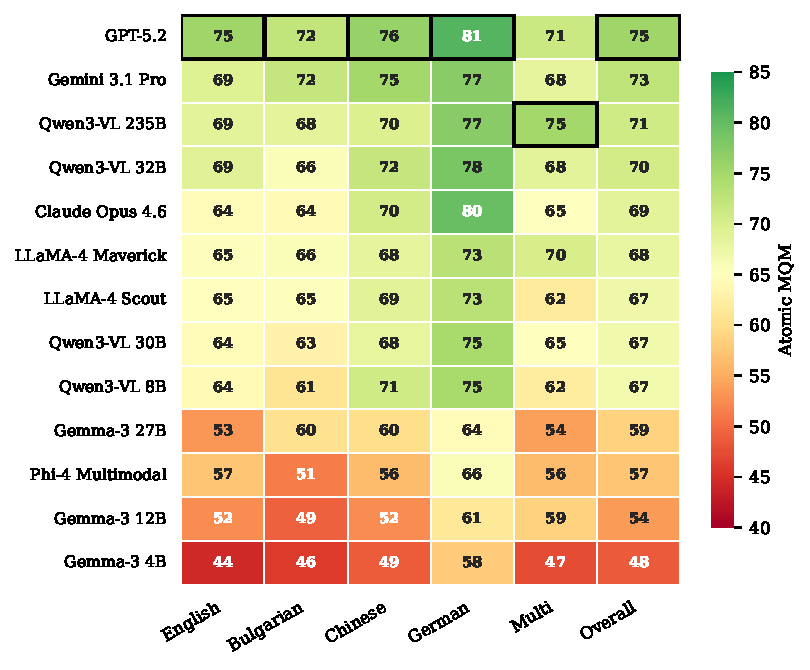
\includegraphics[width=\textwidth]{figures/rq1/heatmap_model_lang.pdf}
    \caption{Model$\times$Language MQM (judge-averaged). Black box = column best.}
    \label{fig:heatmap}
  \end{subfigure}%
  \hfill
  \begin{subfigure}[t]{0.46\textwidth}
    \centering
    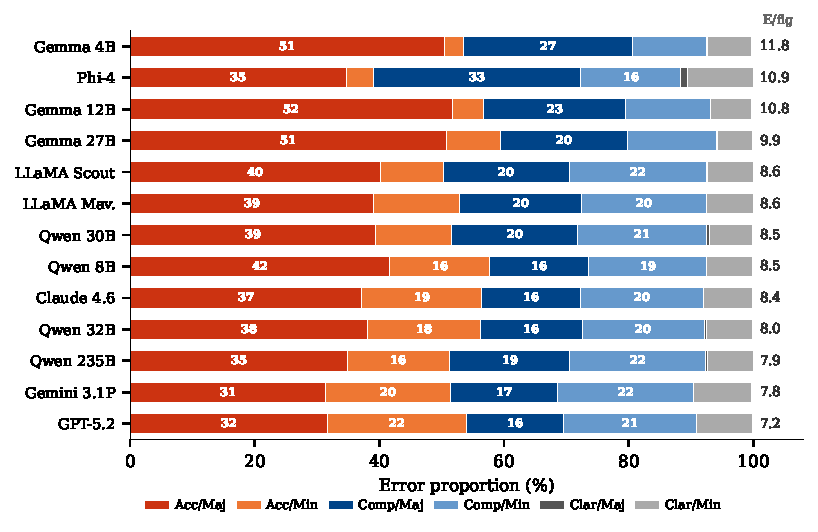
\includegraphics[width=\textwidth]{figures/rq1/error_stacked.pdf}
    \caption{Error composition (100\% stacked). Right = errors/fig.}
    \label{fig:error-stacked}
  \end{subfigure}
  \caption{\textbf{(a)} Per-language performance heatmap. German leads in uncontrolled comparison; the controlled study (\S\ref{sec:rq1-ablations}) reverses this. \textbf{(b)} Error-type proportions per model. Accuracy/Major (red) dominates; weaker models show larger Completeness/Major (blue) shares.}
  \label{fig:heatmap-errors}
\end{figure}

%% -------------------------------------------------------------------
\subsection{Judge Validation Against Human Annotation}\label{sec:rq1-human}
%% -------------------------------------------------------------------

Three annotators evaluated four models on 30~English figures (159~annotations, 39~double-annotated).
Table~\ref{tab:human-judge}(c) reports the results.

The central finding is a \emph{ranking--scoring dissociation}: all evaluators agree near-perfectly on model ordering (system-level $\rho{\geq}.95$, judge--judge $\rho{=}.97$), yet absolute scores diverge by 10--25 points.
Both judges are systematically harsher than humans, with the bias largest for the best model (GPT-5.2: $-$25.6 from GPT-4o) and smallest for the weakest (Gemma-27B: $-$2.2 from Mistral).
This asymmetric compression indicates that judges are more sensitive to minor imprecisions in otherwise strong descriptions.

The two judges diverge primarily in severity assignment: GPT-4o marks 78\% of errors as Major vs.\ Mistral's 47\%, directly inflating GPT-4o's penalty weights.
Averaging two judges with complementary severity profiles stabilises the evaluation.
Human inter-annotator agreement is excellent (ICC\,=\,.91), confirming that the Atomic MQM rubric yields reproducible human judgements.
Figure~\ref{fig:scatter} visualises this relationship.

\begin{figure}[!ht]
  \centering
  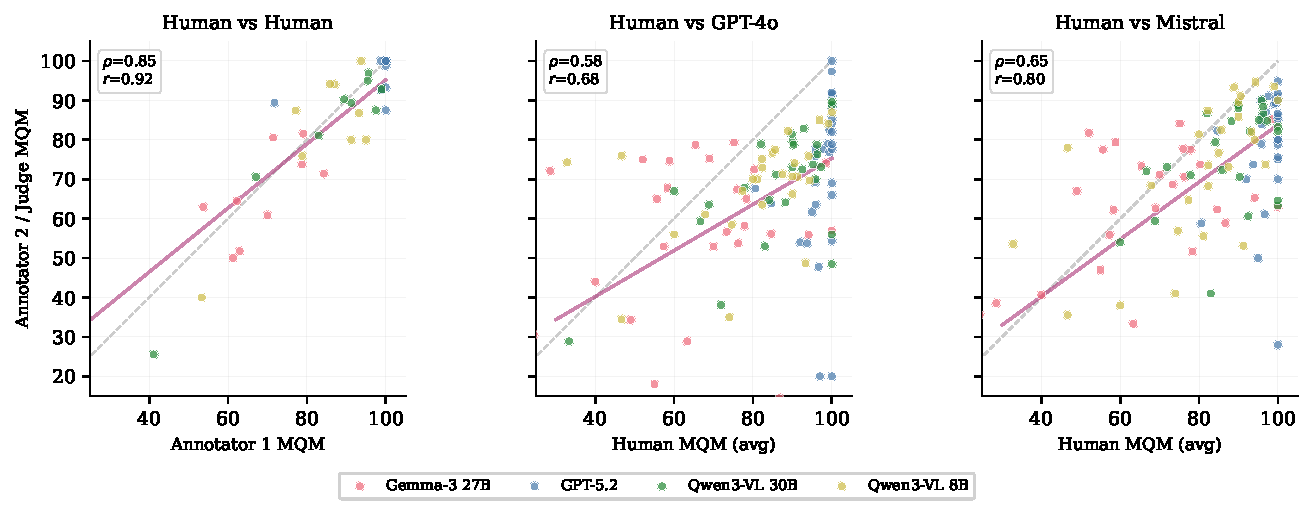
\includegraphics[width=\textwidth]{figures/rq1/scatter_human_judge.pdf}
  \vspace{-8pt}
  \caption{\textbf{Evaluator agreement.} Left: inter-annotator (39 pairs, $\rho{=}.85$). Centre/Right: human vs.\ LLM judge (120 pairs). Dashed = identity; solid = regression. Below diagonal = judge harsher.}
  \label{fig:scatter}
\end{figure}

%% -------------------------------------------------------------------
\subsection{Error Analysis}\label{sec:rq1-errors}
%% -------------------------------------------------------------------

Across 2\,966 evaluations, the judges flagged 26\,364 errors (8.9/fig).
Table~\ref{tab:errors-charts}(b) summarises the aggregate error distribution; the full per-model per-judge breakdown is in Appendix Table~\ref{tab:error-profile-full}.
Accuracy errors dominate, with \emph{Incorrect Numerical Value} alone at 30.6\%, making it the primary bottleneck across all models.
Hallucinated Content, though only 3.6\% of errors, carries 92\% Major severity and correlates inversely with model capacity.
Pie charts score 15--25 points below line/bar charts; the $\Delta_{\text{cap}}$ column in Table~\ref{tab:errors-charts}(d) confirms that ${\sim}11$ of those points stem from multi-error atoms rather than genuine difficulty.
Colour-synonym false positives remain a systematic judge limitation (${\sim}5\%$ penalty on English vs.\ ${\sim}2\%$ on Chinese).
Figure~\ref{fig:error-stacked} shows the per-model error composition.

%% -------------------------------------------------------------------
\subsection{Ablation Studies}\label{sec:rq1-ablations}
%% -------------------------------------------------------------------

\paragraph{Cross-lingual controlled comparison.}
We evaluate 13 parallel figures (same figure, all four languages) with language-specific atom checklists on five models spanning the performance range.
The controlled results \emph{reverse} the uncontrolled language ranking. English scores highest for all models (GPT-5.2 at EN~66.2 $>$ CN~60.8 $>$ BG~56.4 $>$ DE~55.3), confirming that the German advantage in Table~\ref{tab:leaderboard} is a dataset composition artefact.
Chinese is the most resilient non-English language (EN--CN gap 4--17\%), while smaller models degrade disproportionately (Gemma-4B: 42\% EN--DE gap vs.\ Claude's 2\%).

\paragraph{Prompt language (C1/C2/C2\textquotesingle).}
We evaluate three conditions on non-English figures. C1 uses a native-language prompt, C2 uses English for both prompt and output, and C2\textquotesingle{} uses an English prompt with native-language output.
Results are reported in Appendix Table~\ref{tab:app-ablation-prompt}.

\paragraph{Chain-of-thought.}
Compositional CoT prompting~\citep{mitra2024ccot} (``First describe the visual structure \ldots\ Let's think step by step'') is evaluated per model and language.
Results are reported in Appendix Table~\ref{tab:app-ablation-cot}.

